% Chapter 1

\chapter{Introducción general} % Main chapter title

\label{Chapter1} % For referencing the chapter elsewhere, use \ref{Chapter1} 
\label{IntroGeneral}

En este capítulo se presenta el contexto general y la motivación del trabajo realizado.
A su vez, se realiza un análisis del estado del arte relacionado con las tecnologías que se utilizaron
y se establecen los objetivos y el alcance definidos durante su realización.
%----------------------------------------------------------------------------------------

% Define some commands to keep the formatting separated from the content 
\newcommand{\keyword}[1]{\textbf{#1}}
\newcommand{\tabhead}[1]{\textbf{#1}}
\newcommand{\code}[1]{\texttt{#1}}
\newcommand{\file}[1]{\texttt{\bfseries#1}}
\newcommand{\option}[1]{\texttt{\itshape#1}}
\newcommand{\grados}{$^{\circ}$}

%----------------------------------------------------------------------------------------

%\section{Introducción}

%----------------------------------------------------------------------------------------
\section{El desafío de la creación narrativa}

La narrativa\cite{narrative_def} es un género literario que relata un conjunto de sucesos
protagonizados por uno o más personajes y que son presentados a través de un narrador.
Se trata de una forma de expresión cultural fundamental, presente en todas las culturas y épocas,
utilizado para entretener y transmitir conocimiento.
Una de sus características esenciales es la presencia de elementos ficticios, ya sea de manera parcial o total,
con la única excepción del subgénero de crónicas que se limita a relatar hechos reales.
La narrativa sigue siendo un elemento central de la cultura y está
presente en múltiples formatos como la literatura, el cine, la televisión y otros medios tanto físicos como digitales.

La inclusión de elementos ficticios en la narrativa es un proceso creativo
en el que el autor recurre a su imaginación para concebir componentes que, aunque inventados,
resulten verosímiles y significativos.
En este ejercicio mental intervienen múltiples factores, como la coherencia interna y la relación 
entre los distintos elementos que conforman la historia en el espacio y el tiempo.
Estas variables se vuelven especialmente complejas en narrativas con una alta carga ficticia
donde se inventan, además de los personajes y sucesos, contextos completos.
Aquí es donde cobra especial relevancia la construcción de mundos\cite{world_building}, un recurso narrativo fundamental que permite
al escritor diseñar entornos imaginarios detallados y capaces de sostener la lógica del relato.

El proceso de creación de mundos es tan complejo como la narrativa que busca sustentar y
la intención del autor de sumergir al lector dentro de la historia.
En la figura \ref{fig:worldBuildingElements} se presenta una lista amplia, aunque no completa,
de componentes fundamentales en la construcción de mundos 
y la manera en que estos se relacionan entre sí para dar cohesión al conjunto narrativo.

\begin{figure}[htbp]
	\centering
	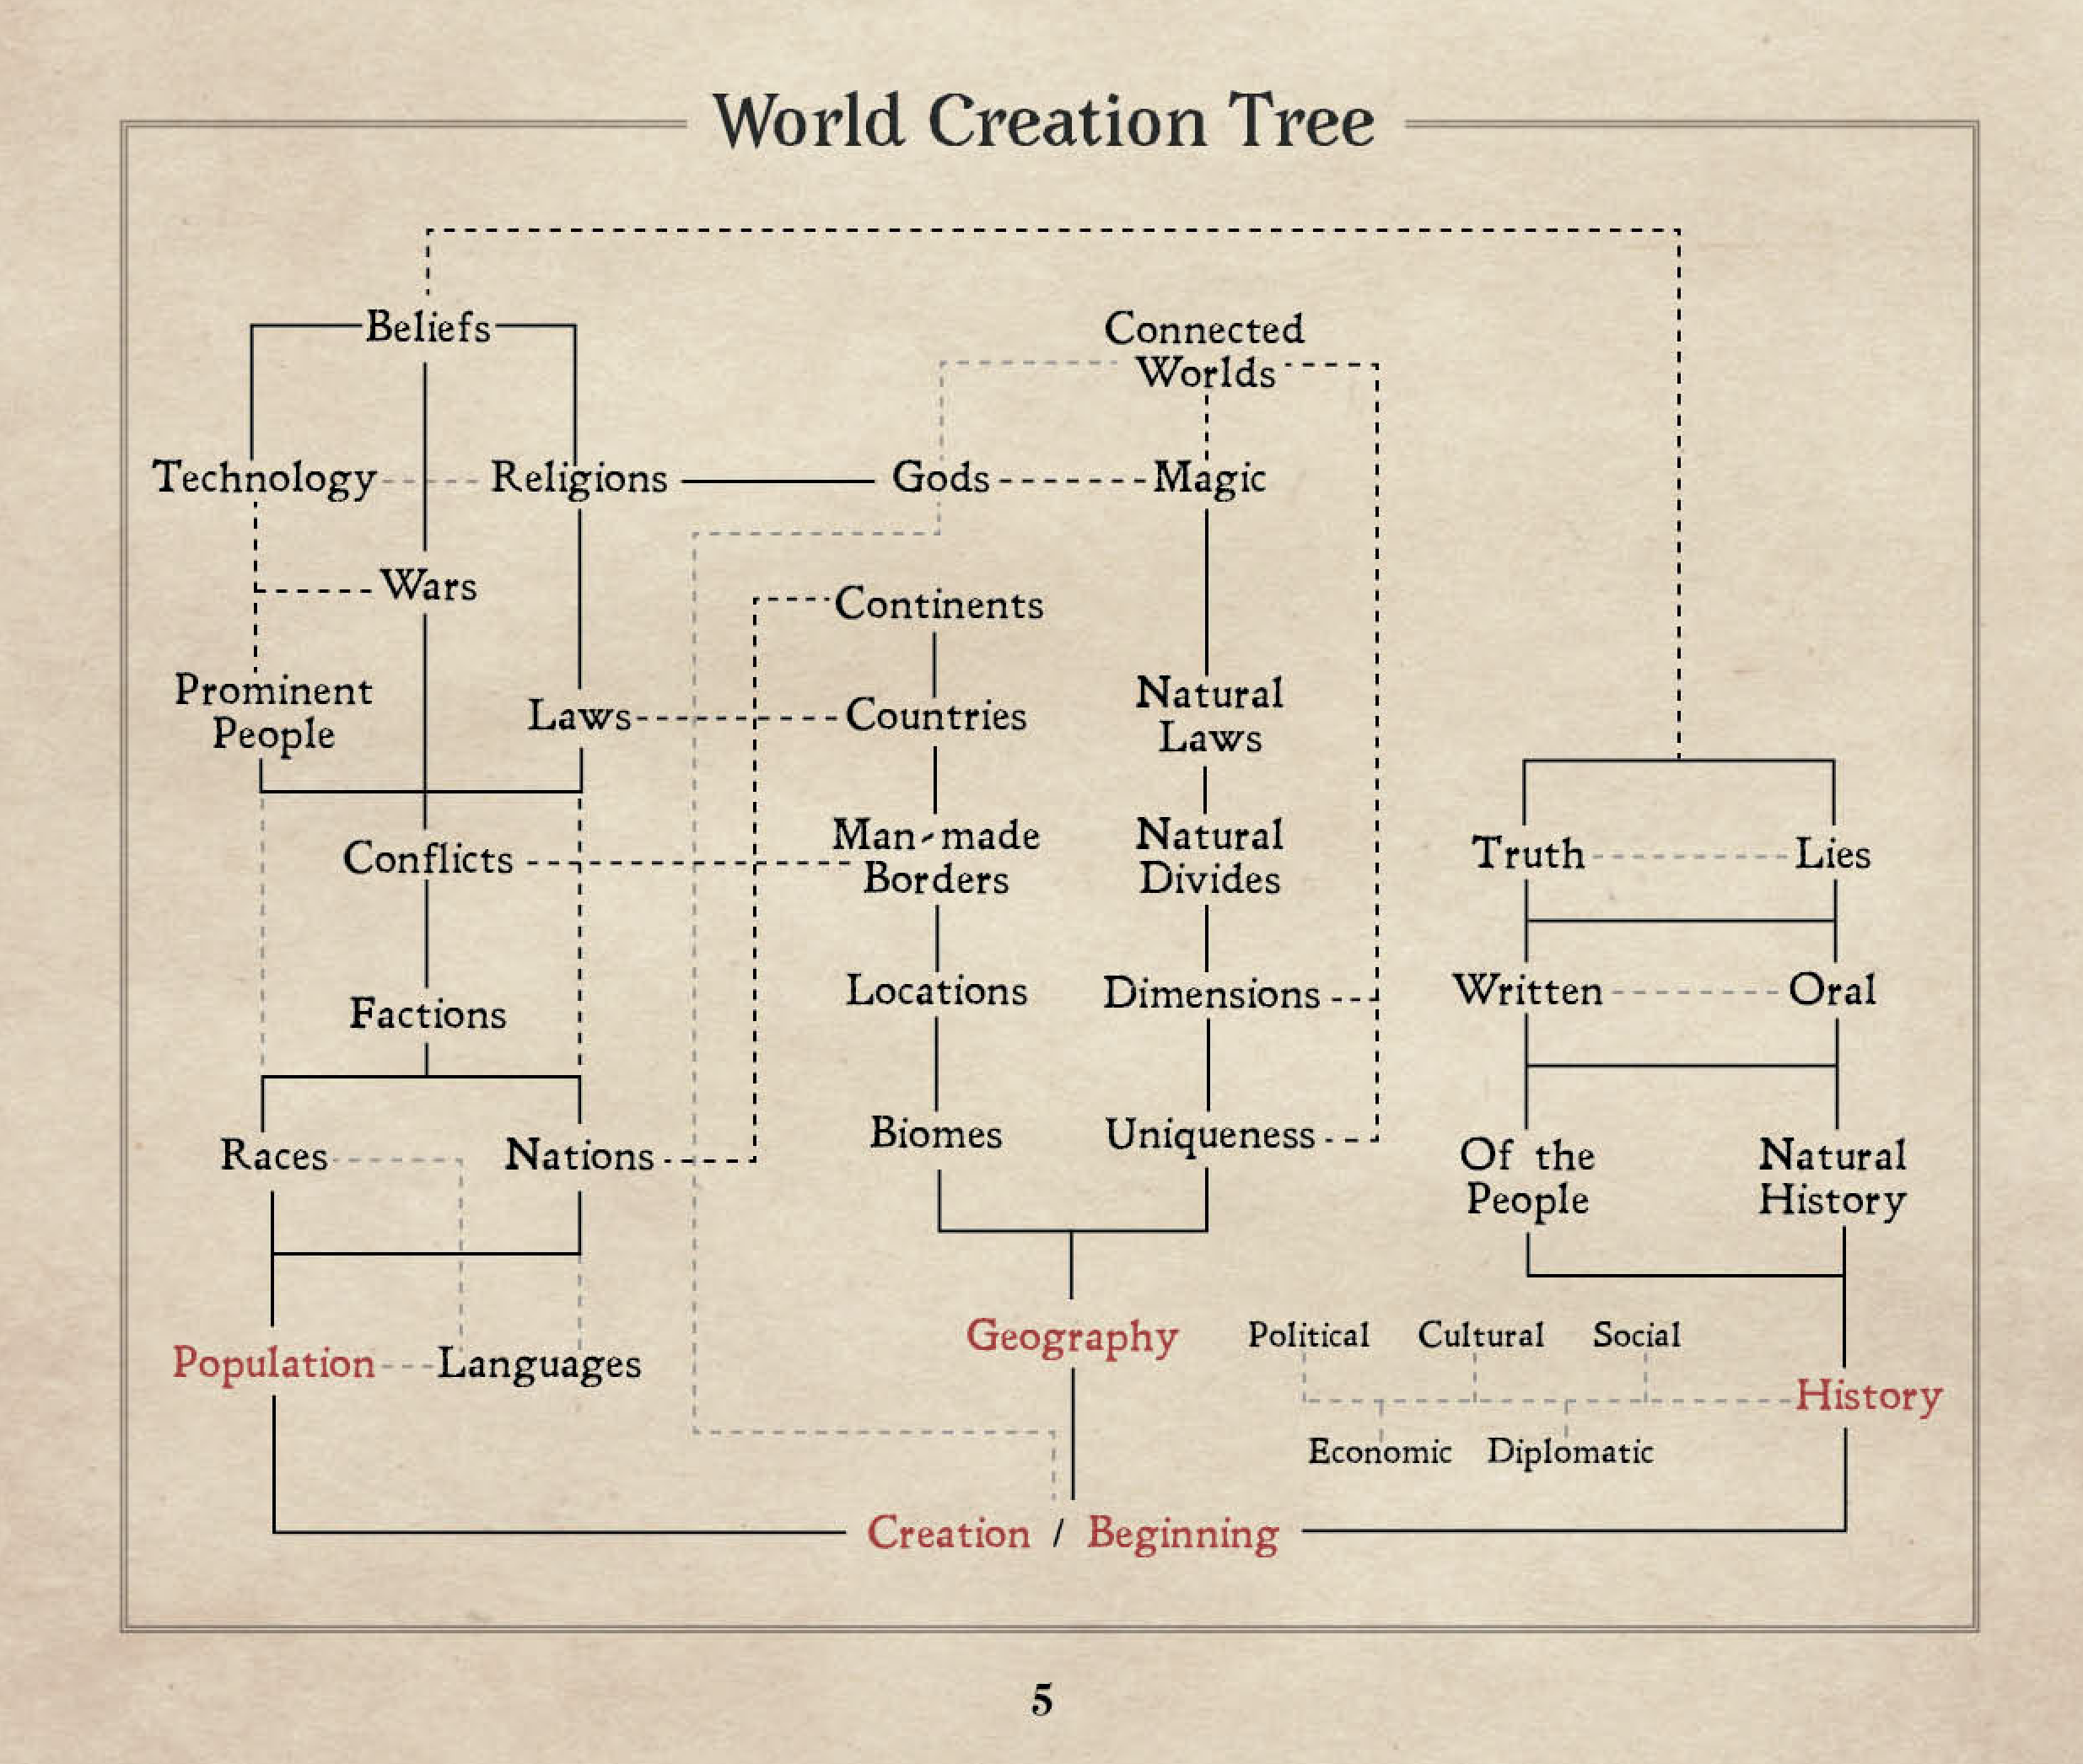
\includegraphics[width=0.9\textwidth]{./Figures/world-building-elements.png}
	\caption{Esquema de elementos habituales en la construcción de mundos}
	\label{fig:worldBuildingElements}
\end{figure}

Históricamente los autores han recurrido a diversas herramientas para llevar a cabo la construcción de mundos,
tales como esquemas, mapas, cronologías, fichas de personajes y la creación de lenguas artificiales.
\footnote{Un ejemplo popular es el de J.R.R. Tolkien, quien creó mapas, genealogías y lenguas para su obra
\textit{El Señor de los Anillos} \cite{tolkien_letters}.}
Todos estos elementos han sido producto del trabajo creativo del autor, apoyado tanto en su imaginación como en la
consulta de múltiples referencias.
Este proceso ha requerido una considerable inversión de tiempo y, en muchas ocasiones,
afectado por bloqueos creativos a la hora de articular y cohesionar todos los componentes ficticios de la narrativa.

En los últimos años la aparición de la inteligencia artificial generativa ha abierto nuevas posibilidades
dentro de los entornos creativos.
Aunque originalmente no fue concebida con fines narrativos, su capacidad para producir texto coherente
la convierte en una herramienta con un alto potencial para incorporarse en la construcción de mundos ficticios.
Sin pretender sustituir la creatividad del autor, estas tecnologías pueden ejercer un papel de apoyo
al facilitar el desarrollo de contenidos y aportar ideas que estimulen la creación literaria.

%----------------------------------------------------------------------------------------

\section{Motivación}
El trabajo se enfocó en la creación de entornos narrativos para juegos de rol 
y surgió de la colaboración con la empresa Critical Match\cite{crit_match_web} y su objetivo de ampliar las herramientas 
y servicios para los usuarios de su aplicación de móvil.
La \textit{app}\cite{crit_match_app} permite la creación y búsqueda de salas de juego que se ajusten a las necesidades y preferencias de cada usuario.
En ese contexto, se busca mejorar la ambientación de las partidas proporcionando al autor de la narrativa a una serie de servicios
para enriquecer el universo narrativo ya creado.

El trabajo aborda la necesidad de los usuarios de conseguir partidas más inmersivas
y reducir el trabajo de ambientación del dueño de la sala de juego.
Reconociendo que no todos los jugadores tienen experiencia con la creación narrativa,
esta herramienta facilita la generación de una ambientación atractiva.
De este modo se optimiza el tiempo de preparación del director de juego, permitiéndole centrarse en otros aspectos de la partida.
Esto también beneficia a los más experimentados al expandir sus ideas con mayor rapidez y eficacia.

Los servicios implementados en el trabajo pretenden ofrecer una experiencia claramente diferenciada de las alternativas más populares en internet
\footnote{Algunos ejemplos son ChatGPT de OpenAI, Gemini de Google o MetaAI.}.
Para ello, se proporciona a los usuarios el acceso a consultas especializadas que solo requieren el envío de un fichero
con la información narrativa, pudiendo combinarse adicionalmente con indicaciones que pueden escribirse en un cuadro de texto.
Este enfoque no solo evita la incomodidad de interactuar con el modelo a través del navegador de internet del móvil,
sino que ofrece respuestas precisas a sus necesidades, que requerirían interacciones complejas
con las alternativas existentes.

Además, este desarrollo se complementa a herramientas existentes de creación de mundos
\footnote{Por ejemplo: WorldAnvil, Obsidian Portal o Legend Keeper.}.
Mientras que estas plataformas brindan la estructura y el marco para la creación de mundos,
el trabajo ofrece la capacidad de generar dinámicamente contenido narrativo específico con la información ya existente.
De este modo los autores a través de ambas herramientas pueden centrarse en la visión general y cohesión del mundo mientras que la inteligencia artificial 
los ayuda con ideas con las que expandir la ambientación, lo que fomenta un proceso cíclico creativo.

%----------------------------------------------------------------------------------------

\section{Estado del Arte}
El avance de la inteligencia artificial generativa ha seguido un ritmo extraordinario desde
la publicación del influyente artículo \textit{Attention is All you need} \cite{att_is_all_you_need}
en 2017.
La arquitectura de los transformadores revolucionó el procesamiento de lenguaje en las máquinas y
permitió paralelizar los procesos a través del mecanismo de atención.
Esto aumenta drásticamente la velocidad y eficacia en el proceso de aprendizaje de los modelos.

En el transcurso del año siguiente surgieron los primeros modelos extensos de lenguaje
que adoptaron la arquitectura de los transformadores.
Con el lanzamiento de GPT\cite{Radford2018GPT1} por OpenAI y de BERT\cite{Devlin2019BERT} por Google, ambos modelos se convirtieron
en los pioneros y pilares fundamentales de los modelos extensos de lenguaje.
Mientras BERT se especializó en la comprensión del contexto del texto de manera bidireccional, GPT
fue desarrollado para la generación de texto.

Desde entonces la evolución de los modelos no se ha detenido. El número de parámetros
ha crecido exponencialmente, lo que les ha otorgado una capacidad sin precedentes para comprender y
producir texto coherente y fluido similar al humano.
Además, este desarrollo ha sido transversal y está dotando a los modelos más recientes 
con la habilidad para generar no solo texto, sino también imágenes, audio e incluso video.

Estos avances están actualmente al alcance del público general a través de internet, con ejemplos destacados
como ChatGPT\cite{OpenAIChatGPT2022}, Gemini\cite{GeminiTeam2023Gemini} o Meta AI\cite{MetaAIAbout}.
ChatGPT fue el pionero y el que abarcó mayor popularidad,
con una interfaz gráfica similar a la de un chat con la que el usuario podía interactuar de forma intuitiva
y sencilla con el modelo. La utilización de estos modelos se masificó rápidamente y se implementaron variantes
en multitud de sectores, principalmente en forma de asistentes virtuales.

En el ámbito creativo, el potencial de la inteligencia artificial generativa es tan amplio como discutido.
Dependiendo de su aplicación, los modelos pueden ser catalizadores del proceso creativo
al ayudar a superar bloqueos y explorar nuevas ideas con rapidez, o bien
reemplazar por completo la labor del artista. 
Este dilema plantea importantes debates sobre la autoría, los derechos de propiedad intelectual 
y el futuro de diversas profesiones creativas.
Actualmente, la relación entre la inteligencia artificial 
y los artistas se encuentra en un proceso de redefinición de su paradigma.

A pesar de sus impresionantes capacidades, 
los modelos generativos se enfrentan a retos muy significativos que se enumeran a continuación:
\begin{itemize}
\item Sensibilidad a los \textit{prompts}:
los modelos generativos son muy dependientes de los datos de entrada.
Pequeñas variaciones en la información inicial pueden llevar a cambios drásticos en el resultado generado,
lo que afecta la precisión de las respuestas y hace que sean menos fiables para usuarios sin experiencia previa.
\item Alucinaciones e inconsistencias a largo plazo:
persisten las dificultades para mantener la coherencia y consistencia
en textos extensos debido a la capacidad finita de su memoria (ventana de contexto).
También existe la posibilidad de que la salida se vuelva incongruente o que se genere información ficticia
debido a factores internos o a la complejidad de la solicitud.
\item Sesgos en los datos de entrenamiento: 
los modelos pueden perpetuar o amplificar prejuicios sociales presentes en los datos con los que fueron entrenados.
\end{itemize}

Para mitigar estos problemas utilizan las siguientes tecnicas:
\begin{itemize}
\item Generación aumentada por recuperación:
esta técnica permite a los modelos consultar fuentes de datos externas 
y ampliar la información de la entrada con elementos que están fuera de su entrenamiento inicial
o de su ventana de contexto inmediata.
Esto reduce las alucinaciones y mejora la verosimilitud de la respuesta.
\item Filtrado de datos de entrenamiento: 
se implementan procesos más rigurosos para limpiar y despolarizar los conjuntos de datos de entrenamiento,
para minimizar la presencia de sesgos.
\item \textit{Fine-tuning}
\footnote{La idea de \textit{fine-tuning} se popularizó enormemente con el desarrollo de los modelos de lenguaje pre-entrenados,
siendo el paper de BERT\cite{Devlin2019BERT} uno de los más influyentes al respecto.}: 
consiste en la adaptación de los modelos a tareas específicas a través de un proceso de reentrenamiento parcial.
\item \textit{Prompt engineering}
\footnote{El concepto de \textit{prompt engineering} se hizo fundamentalmente relevante y visible con la publicación del paper de GPT-3\cite{Brown2020GPT3},
que demostró las capacidades de aprendizaje \textit{few-shot} e \textit{in-context learning} mediante la formulación de instrucciones de texto.}:
se basa en la formulación precisa de instrucciones en la entrada para guiar la generación de la respuesta 
y obtener mejores resultados.
\end{itemize}

Este trabajo se fundamenta en este marco de conocimiento
y se emplearon varias técnicas expuestas para mitigar el impacto de las
limitaciones actuales de los modelos generativos.

%----------------------------------------------------------------------------------------

\section{Objetivos y alcance}
El propósito del trabajo es desplegar un componente que aloje los modelos extensos de lenguaje
con los que generar contenido narrativo a partir de una entrada.
Este servidor también es capaz de administrar los modelos, añadir nuevos y elegir cuáles estarán activos.

A su vez, se dispone de un simple servidor web que actúa como la interfaz gráfica entre el usuario y
la inteligencia artificial. Su función es recibir y mostrar la información al usuario,
procesar sus instrucciones y el archivo adjunto
y transformarlo en una instrucción personalizada según el servicio de generación narrativa solicitado.
Esta instrucción es enviada al modelo de inteligencia artificial generativa, y su respuesta se reenvía al usuario.

Ambos servidores conforman un prototipo de pruebas que se entregará al cliente,
junto con este documento, con el propósito de funcionar como estudio inicial y
como base para futuros desarrollos dentro de su aplicación.

El alcance del trabajo incluye los siguientes elementos:
\begin{itemize}
	\item Desarrollo de un servidor web.
	\item Descripción de los modelos extensos de lenguaje utilizados.
	\item Definición, implementación y descripción del \textit{prompt engineering} para cada servicio.
	\item La integración de un conjunto esencial de servicios REST.
\end{itemize}

El alcance del trabajo no incluye:
\begin{itemize}
	\item Diseño de la página que cumpla con los estándares más habituales.
	\item Securización del servidor web ni de ninguno de sus servicios REST.
	\item Rendimiento de los servicios que garanticen tiempos de respuesta cercanos a tiempo real.
\end{itemize}